\chapter{Fiber-optic sensing}\label{txt.sensing}

Light has revolutionized data transmission and made high data rates possible using optical fibers and laser diodes. Apart from the intended usage, data transmission lines made from optical fibers have a new use case in sensing. The optical fiber can be used to measure useful external properties thanks to the detection and analysis of different light scattering effects of the interaction between the light and the fiber, as discussed in Section \ref{txt.scattering}.

This chapter will discuss fiber optics, optical reflectometry, distributed sensing, and different light scattering effects in the fiber.




\section{Fiber optic sensors}

Fiber optic sensors have three main parts - a \textit{light source}, a \textit{medium} that light passes through, and a \textit{detector}. The principle these sensors use is to generate light at the \textit{source} light (laser diode LD), then passes through the medium, which can be a scanned material or an optical fiber (Section \ref{txt.optical.fibers}). The medium affects the light signal and changes signal properties measured at the detector. This way, fiber optic sensors can detect external properties such as vibrations (seismic, acoustic), pressure, acceleration, rotation, and chemical properties.

There are two types of sensors based on the medium used\footnote{https://www.rp-photonics.com/fiber\_optic\_sensors.html}:
\begin{itemize}
    \item \textit{intrinsic sensors} - the optical fiber is a measuring medium.
    \item \textit{extrinsic sensors} - use optical fiber to get the signal to and from the actual sensor.
\end{itemize}

There are two types of optical fiber sensors based on the location of the measurement:
\begin{enumerate}
    \item \textbf{Point} - These sensors measure only at the location of the transducer\footnote{device transforming energy from one form of energy to another form of energy}
    \item \textbf{Quasi-distributed} - They use many sensors along the fiber to measure 
    \item \textbf{Distributed} - The sensing element is the optical wire. It can measure at thousands of points along the optical wire thanks to different scattering effects, as discussed in Section \ref{txt.scattering}. It can use existing telecommunication infrastructure to build the sensing network.
\end{enumerate}

\subsection{Fiber-optic sensing applications in different fields}\label{txt.sensing.usage}

The advantage of fiber optic sensing compared to other kinds of sensing is that it is immune to signal interference. The optic fiber is made of glass or transparent plastic. It can be used in environments that would be dangerous or harsh for other types of sensors. It is good to mention environments such as flammable, explosive, harsh chemicals, high voltage, or environments that would create electromagnetic noise. Thanks to these properties, fiber-optic sensing has many different applications.

The applications include:

\begin{itemize}
    \item Fiber-optic gyroscopes - rotation measurement thanks to the Sagnac effect. They can replace older ring-laser technology \cite{fog}.
    \item Fiber-optic accelerometers - % TODO .
    \item Fiber-optic bio-sensors - thanks to the chemical and thermal stability of glass fibers, these sensors are perfect for measuring harsh chemicals. Measurements can be done in hard-to-get or small spaces. They also measure on small sample volumes \cite{chemsens}.
    \item Vibration detection - seismic, acoustic,  and even underwater.
    \begin{itemize}
        \item Seismology - measuring and locating earthquakes \cite{dasKislov}.
        \item Building monitoring - bridge monitoring for changes such as cracks \cite{DVSShanFu}.
        \item Perimeter protection - detecting and localizing intrusion into an area, more in Section \ref{txt.perimeter.security}.
        \item Location detection - fiber-optic sensors can detect traffic and vehicles in cities and on highways or locate trains along train tracks \cite{dasKislov}.
        \item Fiber-optic hydrophones - under-water detection systems for seismic monitoring \cite{hydrophones}.
    \end{itemize}
\end{itemize}



\subsubsection{Perimeter security}\label{txt.perimeter.security}

In the early 2000s, perimeter protection using fiber optics was based on breaking or cutting the fiber, triggering an alarm. This is good enough for one-time use because after the wire is broken, there is no choice but to replace or repair the wire. This system can not tell the location when using a single wire. Newer systems used \textit{Sagnac effect}, which uses a Sagnac interferometer and a closed loop made of fiber optic wires, for example, 3x3\footnote{three by three} wire system. Sagnac interferometer detects changes in the phase of light, and thanks to signal processing and calculating the time difference between amplitudes, the position of an intruder is calculated. Such an interferometer has a conversion unit from optical to electric signal. The electric signal is then sampled using a fast A/D converter with high sampling rates. The accuracy of such a system is 20-50 meters which is more than sufficient for perimeter protection\cite{perimeterpolsko}. 

\begin{figure}
    \centering
    \includegraphics[width=\linewidth]{obrazky/sagnac_interrogator.png}
    \caption{3x3 system for perimeter protection using two Sagnac interferometers\cite{perimeterpolsko}}
    \label{fig:sagnac}
\end{figure}

Thanks to research and technological advancements, new devices based on \ac{das} systems are used. These systems use scattering effects that happen in the fiber during the passage of photons through the fiber's medium. These effects are then analyzed at the source of light. The light bounces from imperfections in the fiber and is propagated backward as scattering (\textit{backs-cattering}). Nothing special happens when the fiber is not moving, but when the fiber is affected in any way, for example, by vibrations of an intruder or just by voice alone, the back-scattering changes. These changes can then be analyzed and categorized as an intrusion.


\section{Optical fibers}\label{txt.optical.fibers}


As optical sensing uses existing fiber optic transmission lines, it is important to account for different kinds of optical fibers, materials, and production methods. Optical fibers consist of three main elements \textit{core}, \textit{cladding}, and \textit{coating}. Materials from which core and cladding are made are plastic or glass $Si_2O_3$. 

All-glass fiber dopants, such as $GeO_2$, $P_2O_5$, $B_2O_3$, can be added to all-glass fibers to adjust the refractive index. The core usually has a higher refractive index than cladding by about \qty{1}{\si{\percent}}. Lowering the refractive index can be done by doping fluorine, which is done in the core when the refracting index is too high and needs to be lowered\footnote{https://www.rp-photonics.com/fiber\_core.html}. The radius of core ranges from \qty{3.7}{\si{\micro}\meter} to \qty{200}{\micro\meter} and radius of cladding is up-to \qty{140}{\si{\micro}\meter}\cite{cabling}.

Plastic optics uses organic material in the form of polymers - chains. Materials used are acrylic, polycarbonate, polystyrene, or liquid silicone. The core of plastic fiber has a popular diameter of \qty{980}{\si{\micro}\meter}.

Although the purpose of the coating is simply protection, the fiber would be very fragile without it. It is usually without special color but can be painted to ease the identification of individual fibers. There are multiple layers of coating, at least primary and secondary. The primary coating is softer to allow the bending of the fiber. Secondary is harder to protect inner layers. Materials such as acrylate, silicone, polyimide,e or carbon are used depending on the application of the optical fiber. for example. For example, acrylate has limited temperature resistance; in this case, silicone is better as it is heat resistant up to \qty{200}{\celsius}\cite{cabling}. For more extreme applications, Polyimide is used as it can withstand temperatures up to \qty{350}{\celsius}, and it is also resistant to chemicals and abrasion\cite{cabling}.

% \subsection{Fiber modality}\label{txt.optical.fibers.modality}

% Optical fibers can have different kinds of modality depending on manufacturing processes and desired properties of the material. We differentiate multimode and single-mode fiber optic cables. 

% Multimode optical fibers have much larger core diameter compared to the diameter of cladding. This enables 
% %TODO


% Single mode fibers have single propagation mode  per polarization fir a given wavelength. They have very small core diameter, only few micrometers, relative to the cladding diameter. Since they use only single mode there is no inter-modal dispersion\footnote{https://www.rp-photonics.com/single\_mode\_fibers.html}
% %TODO


\section{Light scattering effects in fiber optics}\label{txt.scattering}

Light precisely photons traveling through a medium - atmosphere, glasses, glass optical fiber, or any other medium can bounce from what is called \textit{scattering centers} in the medium. \textit{Scattering centers} are any non-uniformities in the medium such as vacancy defects (missing atoms in otherwise uniform structure), foreign particles, bubbles, trapped gas molecules, fractures, micro-cracks, any changes in refractive index, density fluctuations, manufacturing imperfections, and others \cite{scatteringcenterbook}. Scattering centers create different kinds of scattering, as will be discussed in the next sections. They include \textit{Mie scattering} (Section \ref{txt.scattering.mie}), \textit{Rayleigh scattering} (Section \ref{txt.scattering.ray}), \textit{Raman scattering} (Section \ref{txt.scattering.ram}) or \textit{Brillouin scattering} (Section \ref{txt.scattering.bril}). For comparison, see Figure \ref{fig:scattering.comparison}. It shows all of these different scattering effects:

\begin{itemize}
    \item 1 - input radiation from a laser diode.
    \item 2 - Rayleigh scattering 
    \item 3 and 4 - Brillouin scattering lines %TODO stokes antistokes
    \item 5 and 6 - Raman scattering 
\end{itemize}

\begin{figure}
    \centering
    \includegraphics[width=\linewidth]{obrazky/scatterings.png}
    \caption{Comparison of different scattering effects \cite{scattering.comparison}}
    \label{fig:scattering.comparison}
\end{figure}

\subsection{Mie scattering}\label{txt.scattering.mie}

\textit{Mie scattering} is an optical phenomenon happening when light traveling through a medium bounces from \textit{scattering centers} the same length or bigger than the wavelength of the light. Mie scattering applies to any spherical particles located in the medium. This also applies to the smaller particles. But we distinguish Mie scattering for particles bigger than the wavelength of light for clarity. For particles smaller than the wavelength of light we distinguish a special case of Mie scattering, and we call it \textit{Rayleigh scattering}, which will be discussed in the next Section \ref{txt.scattering.ray}. That said, there are differences between these two types. The scattered light's amplitudes are stronger for forward scattering in Mie scattering\footnote{https://www.rp-photonics.com/rayleigh\_scattering.html}. Large defects are usually not uniformly distributed along the fiber, which prevents it from being used in \ac{das} systems \cite{dasKislov}.

\subsection{Rayleigh scattering}\label{txt.scattering.ray}

Rayleigh scattering is an optical phenomenon named after British physicist Lord Rayleigh. Light is scattered from scattering centers much smaller than the wavelength of the light, for example, individual molecules or atoms. This is opposite to Mie scattering \ref{txt.scattering.mie}, where light is scattering from larger scattering centers. The difference is that amplitudes are the same for forward and backscattering in Rayleigh scattering\footnote{https://www.rp-photonics.com/rayleigh\_scattering.html}. Compared to other scattering processes, Rayleigh is \textit{linear} scattering process whereas \textit{Raman} and \textit{Brillouin} scatterings are \textit{nonlinear}\footnote{Nonlinear light effects occur when the output intensity does not increase proportionally to the input intensity; for example doubling the optical input intensities does not result in double the output intensity. These nonlinear effects tend to weaken significantly at low optical intensities.}.

Only a small portion of the back-scattered light returns to the source - most of it leaves the fiber on the sides. Rayleigh scattering is used in \ac{das}, as discussed in Section \ref{txt.das}.

When solidified in a medium, not all scattering centers cause Rayleigh scattering. At a wavelength of about 0.95 μm (microns), glass optical fibers have a high attenuation band caused by scattering and absorption by hydroxide ions \cite{scatteringcenterbook}. Silica glass is an amorphous material with random density fluctuations due to its irregular microscopic structure. This can be limited by an annealing process but can not be removed completely\footnote{https://www.rp-photonics.com/rayleigh\_scattering.html}.




\subsection{Raman scattering}\label{txt.scattering.ram}

The effect photons have when interacting with the crystal lattice of glass is called \textit{Raman scattering}. A transparent optical medium, such as glass, has a crystal lattice. The lattice is naturally vibrating, causing a delayed nonlinear response to the light passing through it. The photon traveling through the medium experiences a loss in energy due to interactions with the medium. This is also called \textit{inelastic scattering}. 

% The losses happen as vibration energy is exchanged between what are called \textit{phonos}. 

Raman scattering can be measured by sending two light waves with different wavelengths through the optical medium. The  signal with longer wavelength experiences optical amplification at the expense of the one with a shorter wavelength. This is used in Raman lasers, Raman amplifiers, or Raman spectroscopy\footnote{https://www.rp-photonics.com/raman\_scattering.html}.


\subsection{Brillouin scattering}\label{txt.scattering.bril}


Also known as \textit{Mandelsam-Brillouin scattering} is a scattering effect created when light traveling through a medium is scattered during interaction with thermal vibrations of the medium. The intensity is much lower than Rayleigh scattering; see Section \ref{txt.scattering.ray}. But at the same time, much stronger than Raman scattering. For comparison, see Figure \ref{fig:scattering.comparison}. 

Brillouin scattering in optical fibers primarily occurs in the backward direction, but there can also be some weaker forward Brillouin scattering due to the acoustic waveguide's influence\footnote{\cite{bhundred}}.

Brillouin scattering is used in Brillouin spectroscopy. Thanks to its uniform distribution along the fiber, it can also be used in \ac{das} systems, although it is much weaker than Rayleigh scattering \cite{dasKislov}.


\section{Optical reflectometry}\label{txt.reflectometry}

Optical reflectometry is used for measuring optical cable properties; it can detect defects, joints, breaks, or other damage and their location on the wire. It is the basis for \ac{generalotdr} or \ac{ofdr} and other optical sensors such as \ac{das}. A~pulse of light is sent from the source, such as a light-emitting diode (LED) or a laser diode (LD). The light travels from the source through the optical fiber in pulses and is reflected from the other side of the wire through connections, breaks, damage, or imperfections in the material. All of these create some back-scattering toward the light source \cite{progress}. 


\subsection{Optic Time Domain Reflectometry}\label{txt.reflectometry.otdr}

\ac{otdr} is the most widely used method. When a strain is applied to the fiber, it causes phase-shift changes in the light signal. Provides high sensitivity, resolution, and high sampling rates in the frequency range between hertz and kilohertz. \ac{otdr} has limitations in measuring slowly changing effects and noise components.

\subsection{(\acs{otdr})}   %\acl{otdr} \label{txt.reflectometry.otdr2}

%TODO
https://www.flukenetworks.com/expertise/learn-about/otdr


\subsection{OFDR}\label{txt.reflectometry.ofdr}

\ac{ofdr} analyzes interference of signal between the initial signal and the back-scattered signal but focuses on the frequency scan. A~source of light has to be a laser diode that can be precisely tuned to a certain frequency. The signal given by \ac{ofdr} contains frequency information that can be processed with the Fourier transformation. The output would be the position of the reflective elements along the fiber length. There are also other methods to measure light properties such as \textit{C-OFDR} - coherent version of OFDR using light with the frequency with linear dependency but having problems with high noise levels, and \textit{DSS} - Mandelstam-Brillouin \cite{kislov_das_newparadigm}.

\section{Distributed Sensing}\label{txt.distributed}

Distributed sensing (in general) is a technology using optical fiber as an array of sensors. It was started from the field of optical reflectometry. There are thousands of virtual sensors along the optical fiber. These sensors are not real devices but rather a clever way of measuring differences in the light signal properties, such as changes in phase. It can measure tension, compression, temperature, vibrations, and other strain impacting the fiber and, consequently, the light passing through it \cite{dasKislov}.

We distinguish multiple distributed sensing systems depending on what is measured:
\begin{itemize}
    \item \emph{Distributed Acoustic Sensing} (DAS) - recording sound and vibrations
    \item \ac{dvs} - vibration detection
    \item \ac{dss} - twisting, pulling, bending
    \item \ac{dts} - temperature measurements
\end{itemize}

In this work, we will focus on \ac{das} rather than the other Distributed sensing methods because the \ac{das} is used for the measurements. That said, other Distributed sensing methods are quite similar.


\subsection{Distributed Acoustic Sensing}\label{txt.das}

Implementation of \ac{das} system is usually done by \ac{generalotdr}, \ac{ofdr}, or analysis of other light properties such as polarization and back-scatter correlation. \ac{das} allows the measurement on thousands of points on an optical wire without the need to cut the wire or have multiple sensors distributed along the wire. The measurement mechanism is based on optical reflectometry, the same as in \ac{dts}, a variant of \ac{generalotdr}. \ac{das} relies on non-uniformities spread evenly along the fiber. As discussed in Section \ref{txt.scattering.ray}, the best suited for this application is Rayleigh scattering, which describes light scattering from particles smaller than the wavelength of the light. In this case, the particles are molecules and atoms in the fiber itself.

During measurement, pulses of light are sent into the optical fiber. The fiber creates a light scattering (e.g., Rayleigh scattering) in the glass that travels back to the sensing unit (on the same side as the light source), which can be interpreted based on the arrival time as a position on the wire. Back-scattering light from the optical fiber segment is detected at the light source. If a strain or a vibration is applied to the optical fiber, it detects changes in amplitude or phase, which means that the fiber wire segment is externally affected somehow. \ac{das} is used in a wide range of applications, from locating seismic activity, locating trains along the train tracks, as a~gyroscope or an accelerometer or even as a~microphone \cite{WangYu2017RDVM}, \cite{kislov_das_newparadigm}.

\ac{das} uses optical fiber as many sensors along its length. The fiber is  capable of detecting vibrations along it can also detect acoustic properties as they are also vibrations but of sound. These sensors allow for measuring acoustic properties such as frequency, amplitude, and phase \cite{WangYu2017RDVM}. 


\subsection{iDAS}\label{txt.idas}


The distributed acoustic sensor is a~new addition to distributed optical fiber sensors used in the energy industry and can be used in many applications, for example, in detecting seismic activity. iDAS (intelligent distributed acoustic sensor) is one type of DAS sensor. One of the applications of this sensor is to record an acoustic signal. To determine the signal fidelity, a certain part of the wire is subjected to a known signal, e.g. sine wave. A measurement is made, and the result is compared with the existing recording device. The result suggests that iDAS has very good signal properties. The measured signal shows that almost no measurable crosstalk is exhibited between the two sensing channels on the wire.

The maximum sampling rate can be calculated from the speed of light that travels in glass at a speed of about \qty{200000}{\km/\s}, which corresponds to approximately \qty{10}{\kHz} for \qty{10}{\km} long wire \cite{WangYu2017RDVM}.

% 10 kHz == 10 km, 1 kHz == 100 km [doplnit vzorcek]

\begin{itemize}
    \item Acoustic bandwidth
    \item Dynamic range - \qty{120}{\dB} as reported in \cite{dasseismic}
    \item Spatial resolution - about \qty{1}{\m} to \qty{10}{\m}, but up to \qty{25}{\cm} is possible
    \item Measurement range - The fiber length can be anywhere from a few hundred meters to more than \qty{100}{\km}.
\end{itemize}


\section{OptaSense ODH-F}\label{txt.optasense}

Data used in this project are obtained from \textit{OptaSense ODHF Distributed Acoustic Sensing Interrogator}\footnote{\url{https://www.optasense.com/technology/odhf/}}(Interrogator). This device is capable of monitoring optical fiber up to \qty{50}{\km} long (in qualitative mode). It is used for in-well flow monitoring, pipeline integrity management, and border security. OptaSense comes with \textit{DxS Visualization Software} capable of analyzing and processing output data from the unit. It can show the signal spectrum in a waterfall graph and create analysis, process the signal using \ac{fft}, and extract data to \verb|.wav| format. It has the limitation that it can only run in the Windows ecosystem and is proprietary software, so scientists cannot really change how they work with the data or how it is displayed.


\subsection{HDF5 file format}\label{txt.hdf5}

The data captured by the Optasense Interrogator is collected in \ac{hdf} and saved into a file with \textit{.h5} suffix. \ac{hdf} creates a model for managing and storing data. The HDF Group\footnote{\url{https://www.hdfgroup.org/}} maintains the format and its corresponding software package. Specifically, the \ac{hdf} format is used to store data, but only one of the three parts makes up the full \ac{hdf} model. Parts of the \ac{hdf} model are:

\begin{itemize}
    \item File format - files ending with .h5
    \item Data model - specifies the building blocks of the \ac{hdf} file format
    \item Software - libraries, tools, APIs
\end{itemize}

\bigskip

\ac{hdf} data model has a folder-like organization, where the folders are called \textit{groups}. This model specifies the format in which the data are stored in the form of \ac{adm}, which specifies the organization of the data and the types of data. Every \ac{hdf} file has to have a~root group \textit{``/''}. Working with groups is very similar to directories on Linux systems; see Section \ref{dir:filestructure}. Each group can have \textit{datasets} that contain raw data, attributes, data types, and other objects. \ac{hdf} file can also specify links to other libraries and tools such as compression and filtering.

\bigskip
HSDF5 dataset has connections with other HDF5 objects:

\begin{itemize}
    \item \textbf{attributes} - named data object containing the name and the value
    \item \textbf{datatypes}:
    \begin{itemize}
        \item Atomic datatypes - time, string, integer, float.
        \item Composite datatypes - array, enumeration, compound, variable length.
    \end{itemize}
    \item \textbf{data} - data itself, for example, the result of measurement.
    \item \textbf{dataspace} - the shape of the data.
\end{itemize}


\begin{figure}
    \centering
    \includegraphics[width=\linewidth]{pdf/hdf5_file_structure.pdf}
    \caption{Basic HDF5 file structure}
    \label{fig:filestructure}
\end{figure}

\newpage

\section{Existing technology for data visualization}\label{txt.design.existing}

This section focuses on data processing and visualization using existing software for visualizing scientific data. First is OptaSense OS6 software which is a purpose-made solution for OptaSense devices. Next is the h5web library, written in React, which creates a web page for visualizing the content of HDF5 files.

\subsection{OptaSense OS6}\label{txt.design.optasense}

The OptaSense company provides visualization software for their devices called OptaSense OS6\footnote{\url{https://www.optasense.com/technology/os/}}. It supports only Windows operating system. OS6 provides features for monitoring areas or land, for example, a compound or an industrial building. This product is tailor-made for OptaSense devices by the OptaSense company. This system has only one window for everything. The primary view is the monitored area; the background picture is the aerial view of the monitored space, as seen in the picture \ref{fig:ossix}. The user can open the sidebar on the right side. The sidebar provides multiple different options:

\begin{itemize}
    \item \textbf{Spectrogram} - Raw data visualization.
    \item \textbf{Alerts} - When an action is detected along the wire, it is logged.
    \item \textbf{Notifications} -  Notifications about system state.
    \item \textbf{System status} - Overview of all OptaSense units and their state.
\end{itemize}

There is also a feature that takes raw data from interrogator units and processes them using machine learning. This way, different actions are detected and categorized into different alerts, such as walking, driving cars, etc. In addition, the user can see the activities detected and triggered in the area overview with live monitoring and a timeline at the top of the screen. To easily look at different locations or start a new view, a feature \textit{type to search} lets the user start a search by typing into the view. For example, the user starts writing ``water...'' as a waterfall, and the program will look for this feature and open the waterfall visualization window. OS6 saves all detected activities, shown in the \textit{Historic timeline} window, which shows all alerts during a specified time range. The animations look very nice, although some look choppy, mostly when showing activities on top of the waterfall view. 

It proves that it is possible to create a real-time data visualization from the \ac{das} system. It lacks one important step, which is the ability to be used not only on Windows machines and be multi-platform. And although it provides enough tools for data analysis, it is unsuitable for further scientific work such as custom editing the visualization or exporting data to images and further processing for machine learning and activity categorization.

\begin{figure}[t]
    \centering
    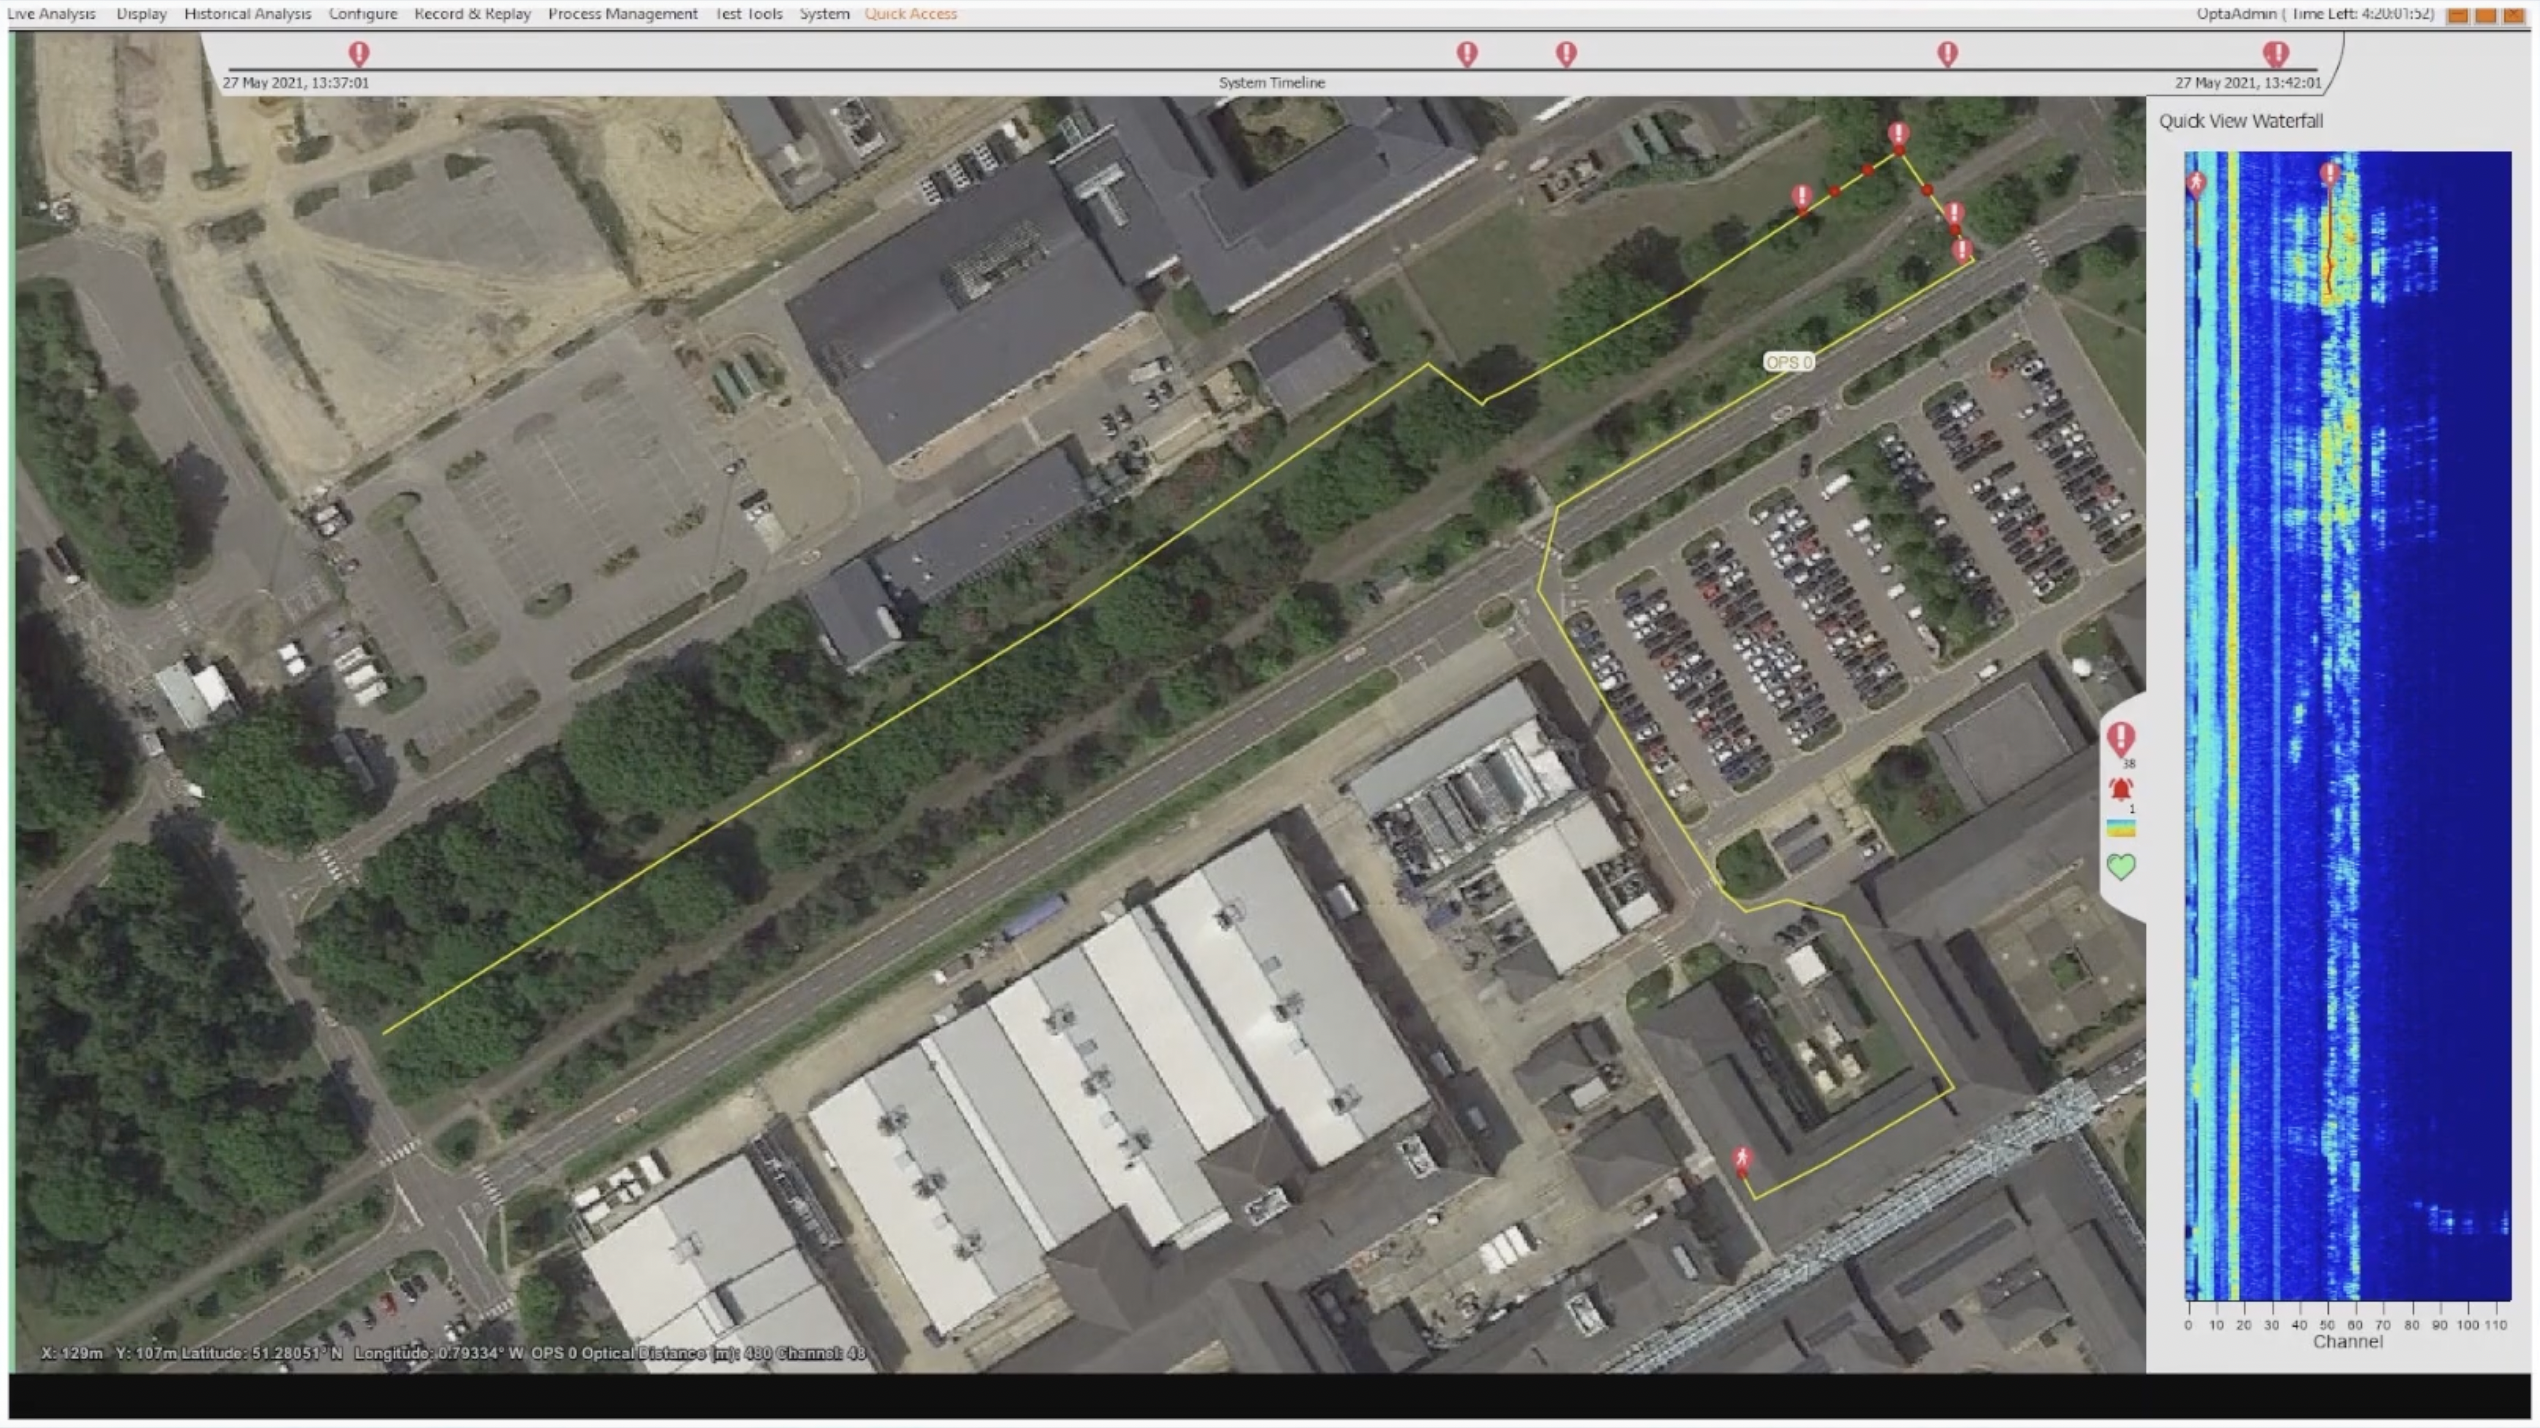
\includegraphics[width=\linewidth]{obrazky/OSsix.png}
    \caption{OptaSense OS6 visualization software \cite{ytossix}}
    \label{fig:ossix}
\end{figure}


\subsection{h5web}\label{txt.design.h5web}

The \verb|h5web|\footnote{\url{https://h5web.panosc.eu/}} library is a set of components written in React\footnote{React is a JavaScript library used to create interactive user interface \url{https://reactjs.org/}}. H5web uses existing HDF5 libraries, such as h5wasm (reading HDF5 files in the browser) and h5grove (server for accessing HDF5 files). It displays the contents of the HDF5 file and shows different graphs according to the input from the user. From the presentation of the library by its developer, it is safe to say that although it provides the necessary equipment for opening HDF5 files elegantly and provides advanced graphing techniques, it lacks the ability to receive the data and display them as they were coming from the \ac{das} system. For this purpose, the library would need to add support by creating a new React component capable of such behavior.

\begin{figure}
    \centering
    \includegraphics[width=\linewidth]{obrazky/h5web.png}
    \caption{h5web application with an example data visualization}
    \label{fig:h5web}
\end{figure}

\newpage